In the following section we will present our results from the implementation and evaluation. For accessing the potentials and limitations of integrating LLM based Automated Bug Fixing into software development workflows using Continuous Integration we implemented a working prototype. During the implementation \ref{chapter:implementation} all self developed requirements \ref{chapter:requirements} are satisfied.

The application of the prototype on a real Github repository \ref{section:evaluation} is demonstrated in the first part of this chapter by showcasing the resulting workflow on GitHub. In the second part of this section we  present the results of the quantitative evaluation the prototype being used on the prepared mentioned repository containing the QuixBugs benchmark.

\section{Showcase of workflow} \label{section:showcase}
%TODO add borders to figures
Setting up the APR system in a repository is archived by adding 2 required files and one optional configuration file to the repository. As seen in \ref{fig:setup} the required files are the \textbf{.github/workflows/auto-fix.yml} file and the \textbf{.github/scripts/filter\_issues.py} file. The optional configuration file is the \textbf{.bugfix.yml} file.

\begin{figure}[H]
    \centering
    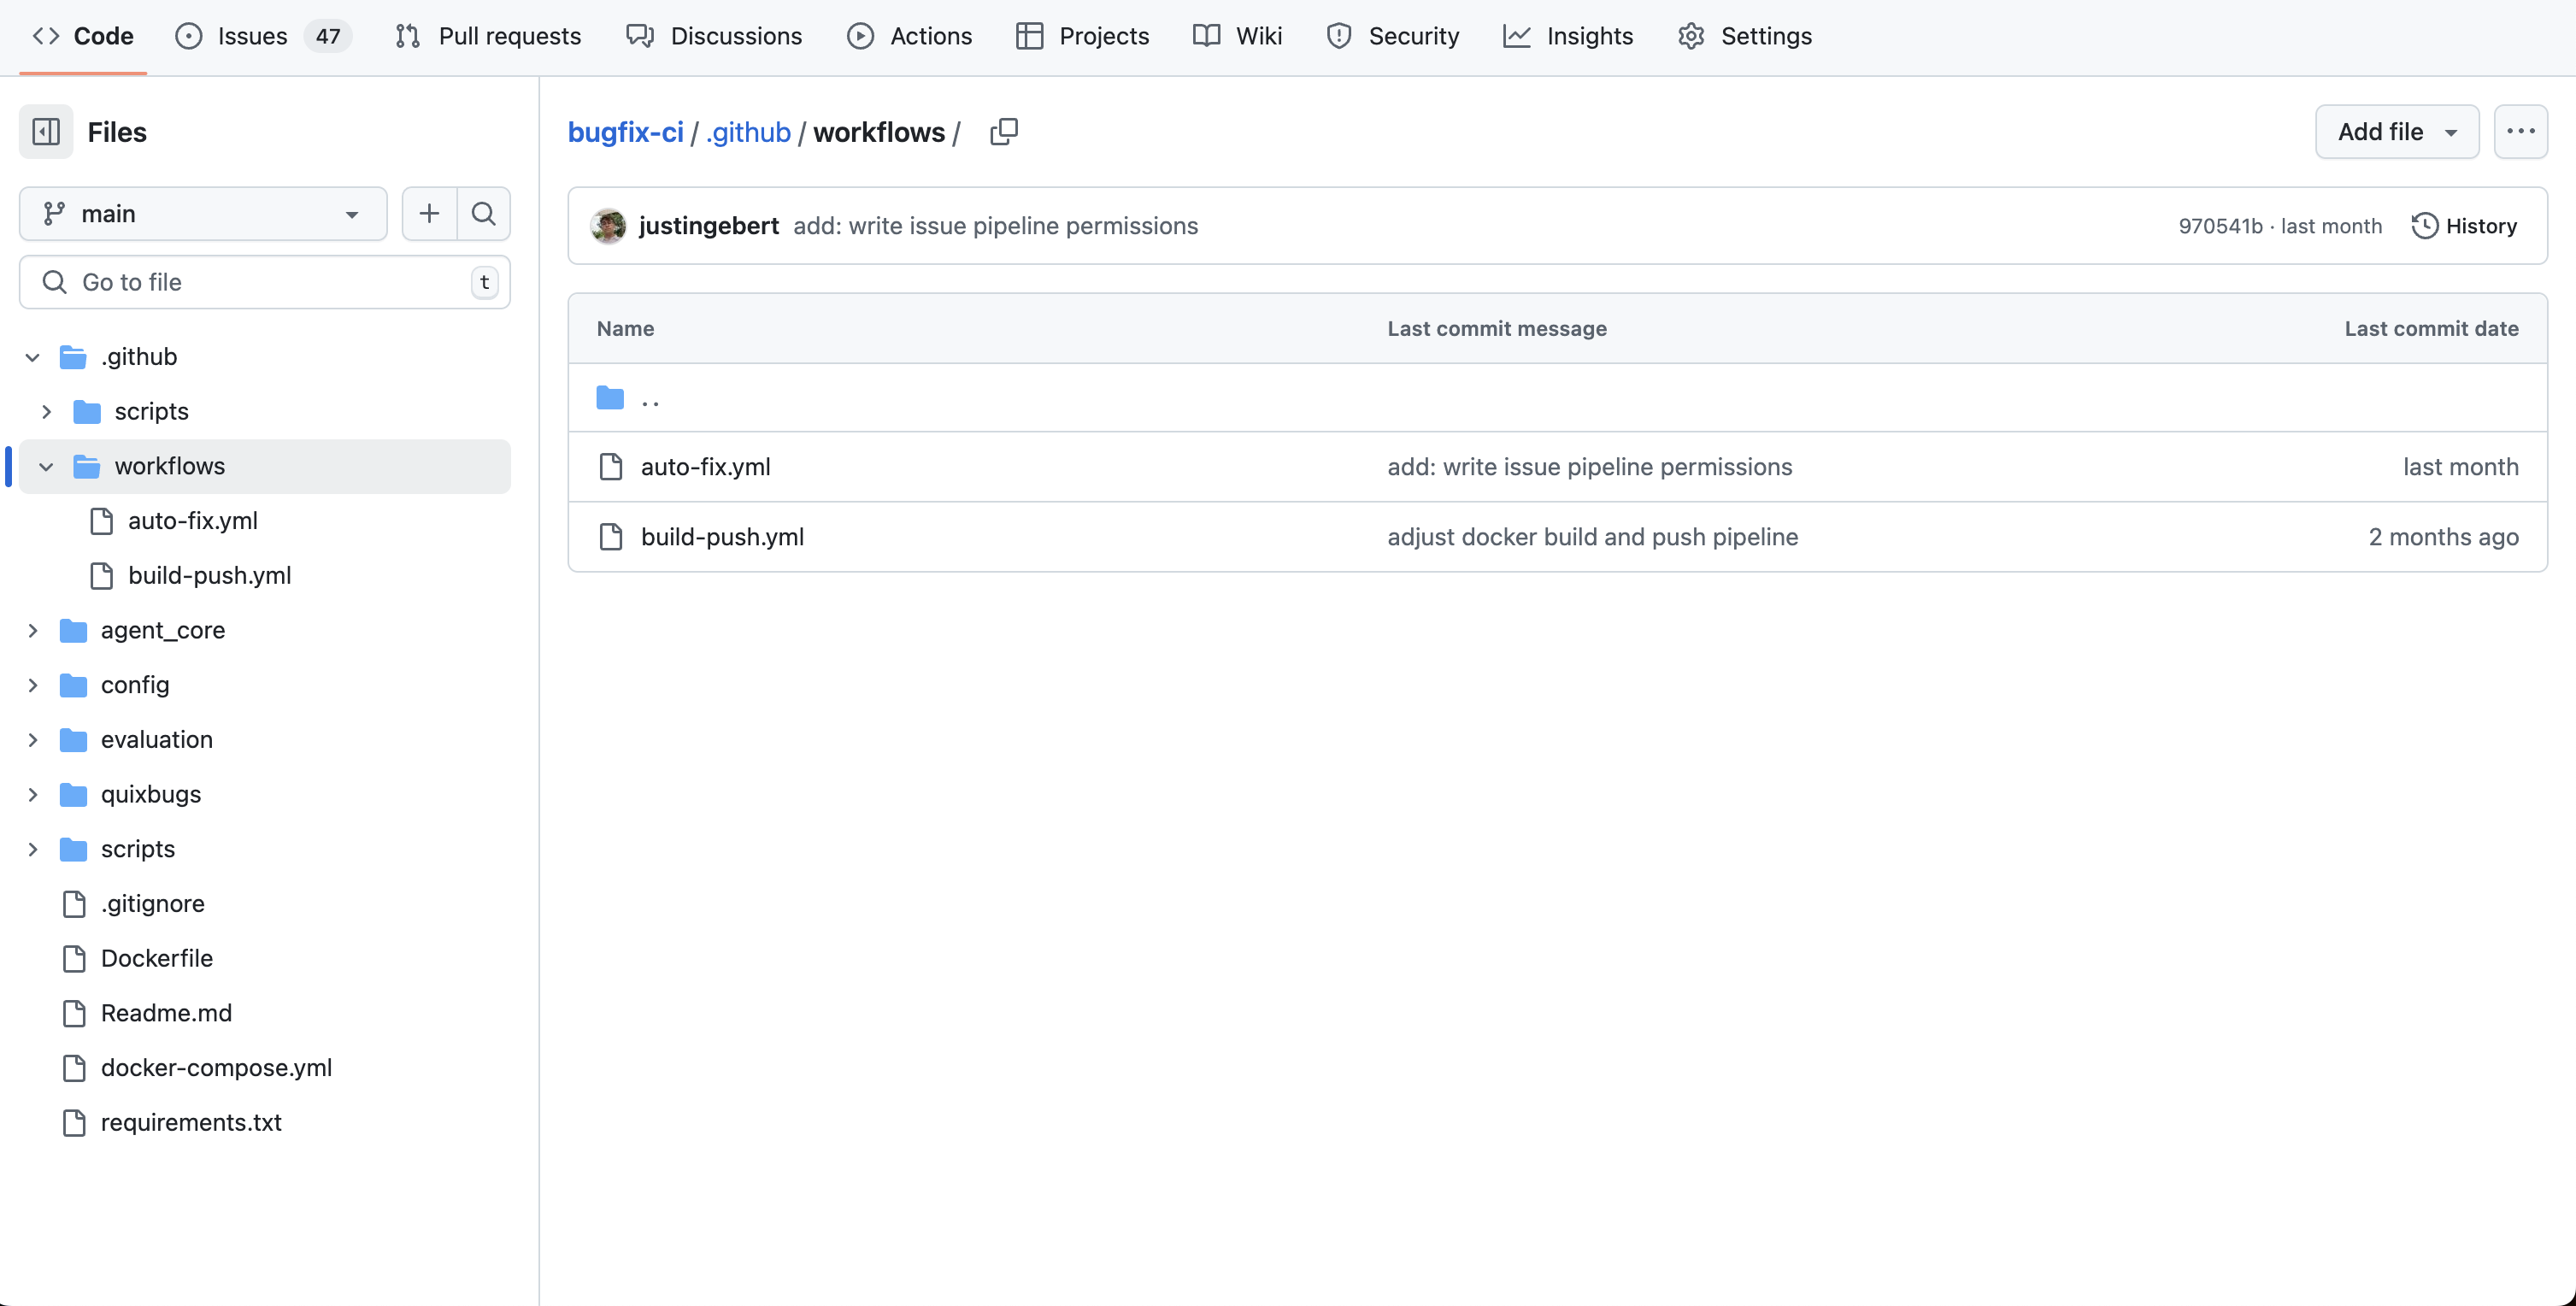
\includegraphics[width=1\textwidth]{images/workflow/setup.png}
    \caption{Set up of APR in a repository}
    \label{fig:setup}
\end{figure}

With the system in place and a custom configuration file set up, the APR system is ready to be used in the repository. Automated bug fixing can be applied in two ways.
Processing one issue per run by labeling the issue with the with the default (bug\_v01) or configured label will trigger the workflow and process the issue. This allows for fast feedback and quick bug fixing at issue creation
\begin{figure}[H]
    \centering
    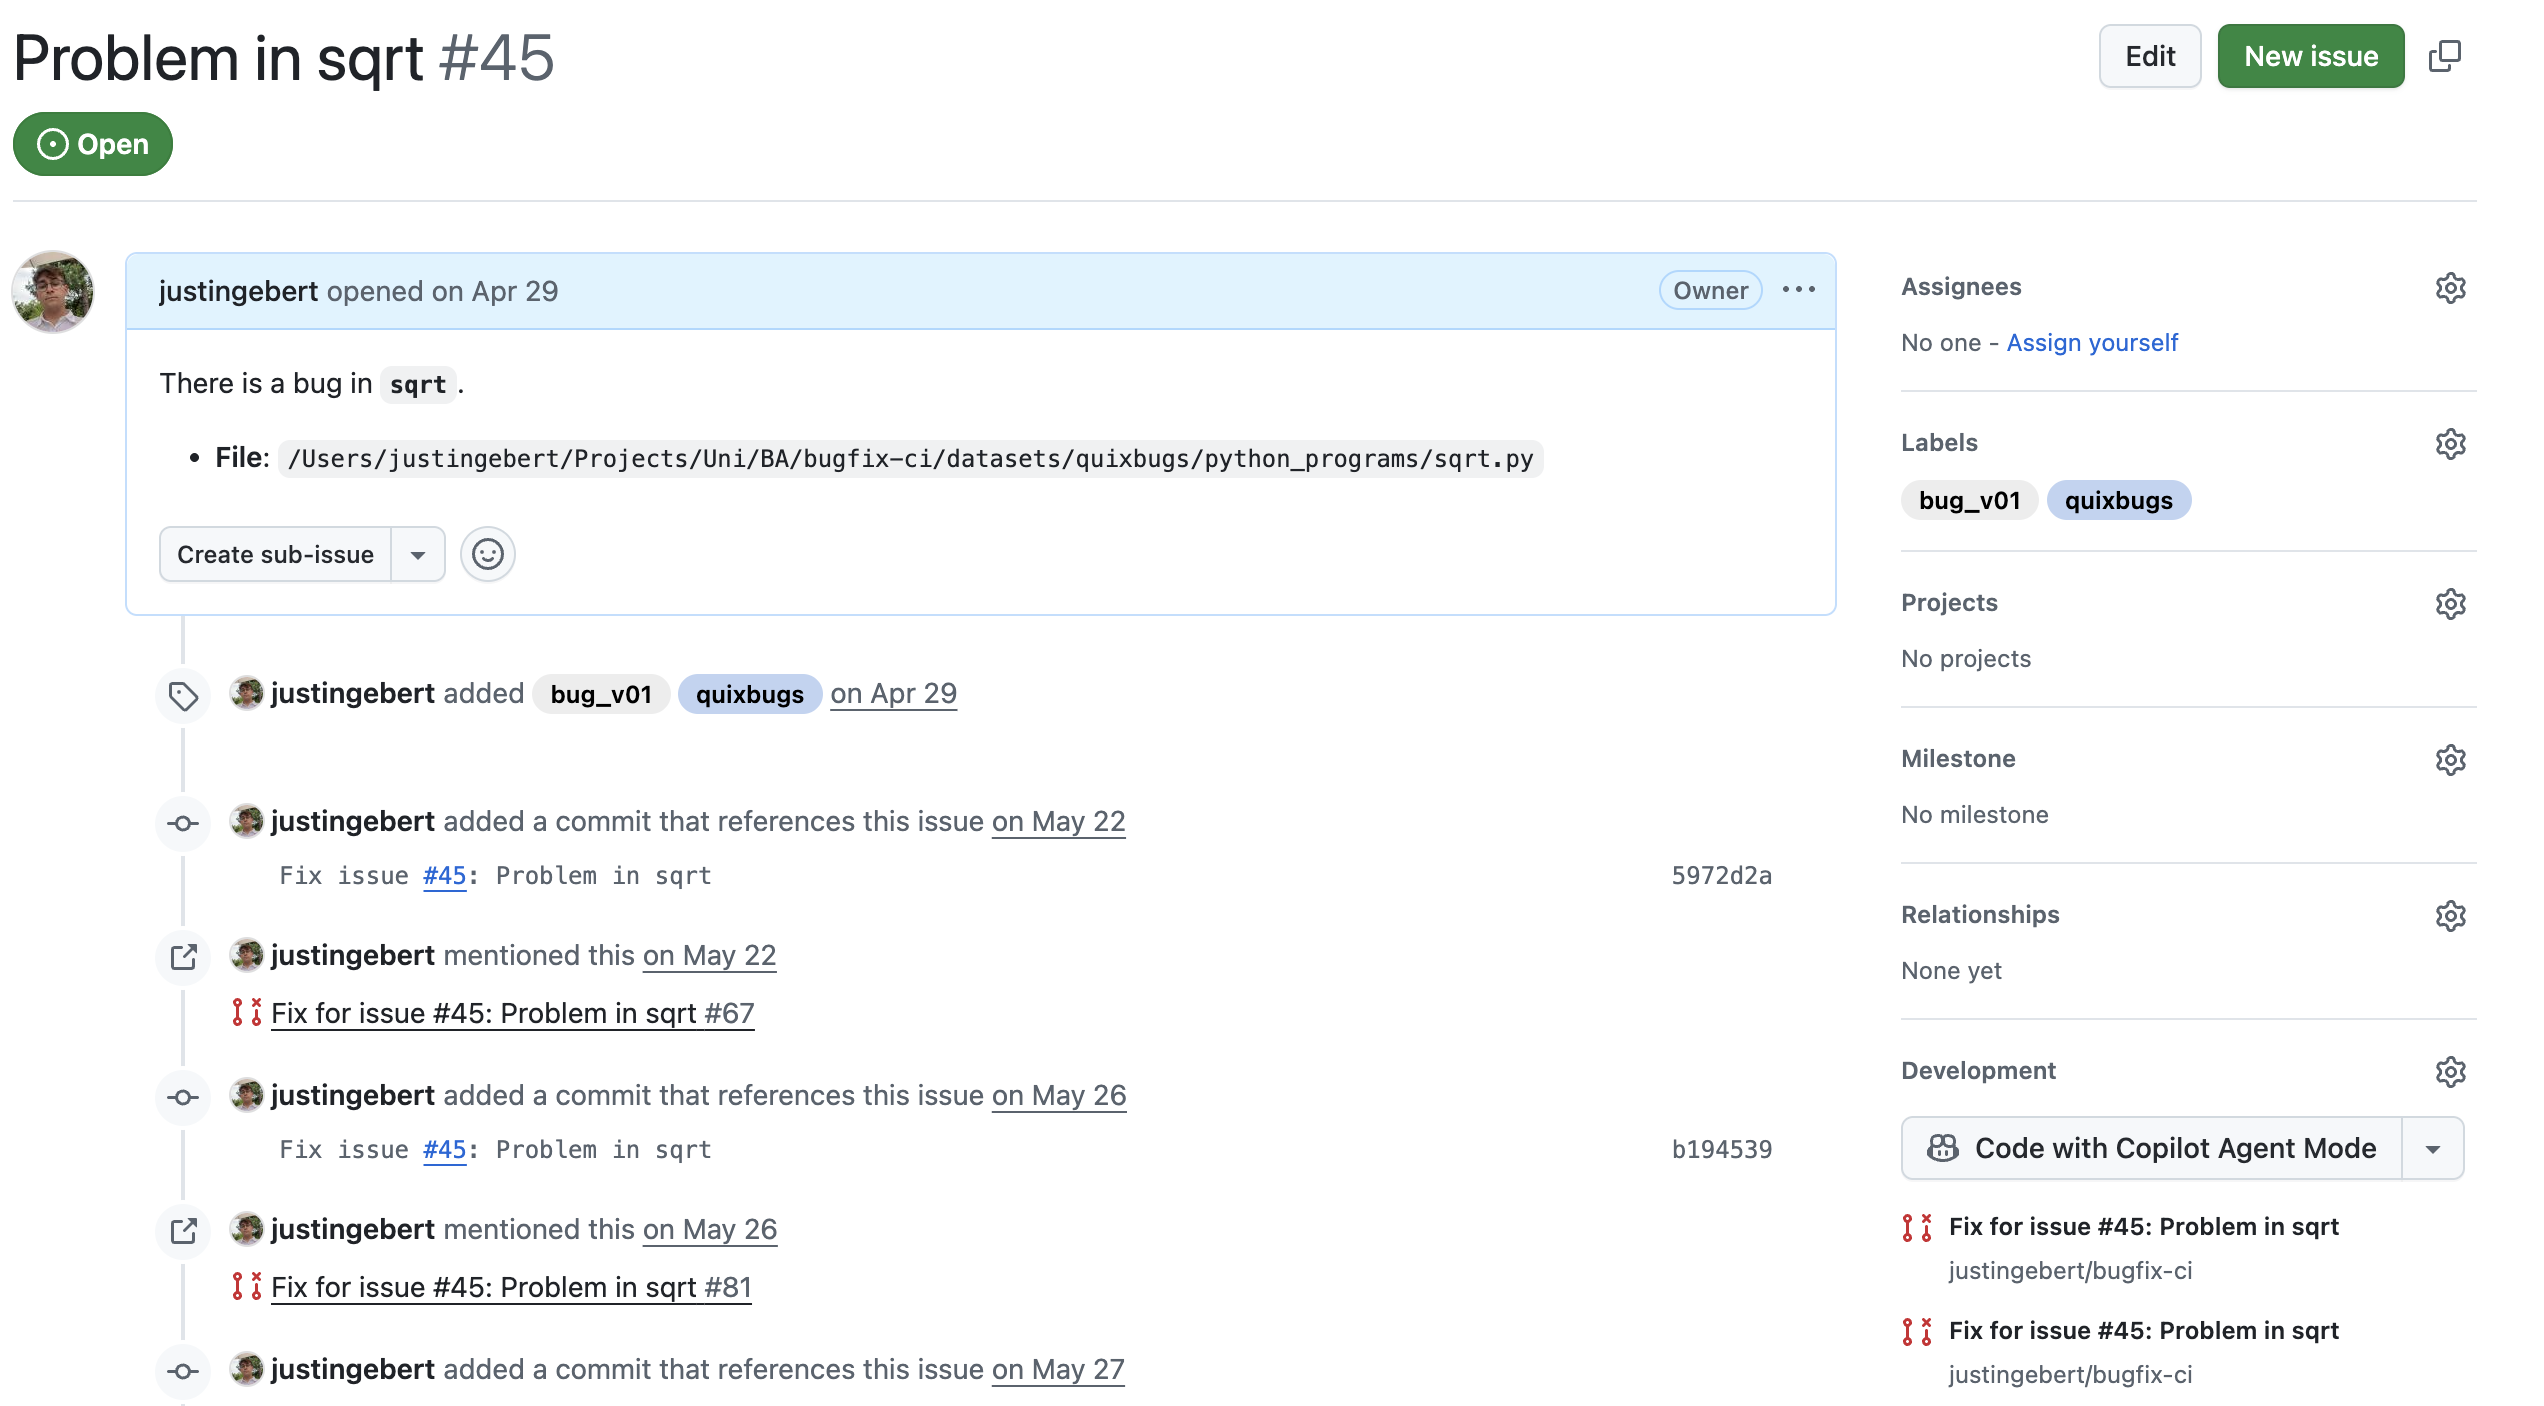
\includegraphics[width=1\textwidth]{images/github/GitHub Issue.png}
    \caption{Trigger automatic fixing for single issue}
    \label{fig:issue-trigger}
\end{figure}

The second way is to process all issues labeled with the default (bug\_v01) or configured label by scheduling the workflow to run at a specific time or dispatching it manually. This allows for a more automated approach to bug fixing, where issues are processed in batches.
\begin{figure}[H]
    \centering
    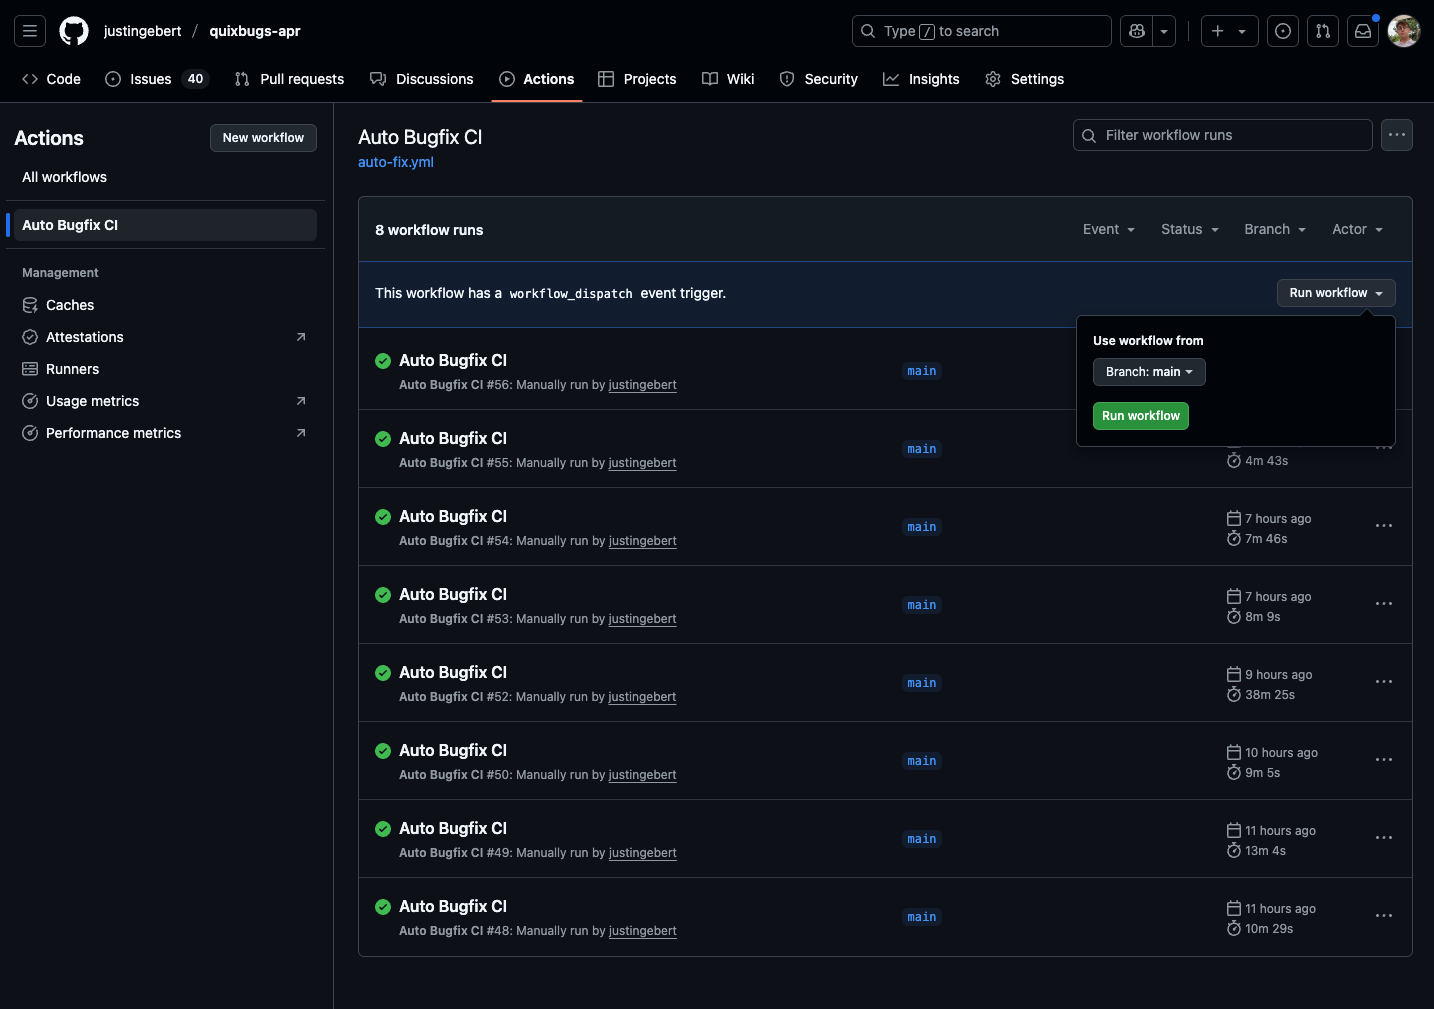
\includegraphics[width=1\textwidth]{images/workflow/dispatch.png}
    \caption{Manual Dispatch of APR}
    \label{fig:dispatch}
\end{figure}

When the workflow is triggered it will create a new run in the GitHub Actions tab. This execute the relevant steps previously described in \ref{chapter:implementation}.

\begin{figure}[H]
    \centering
    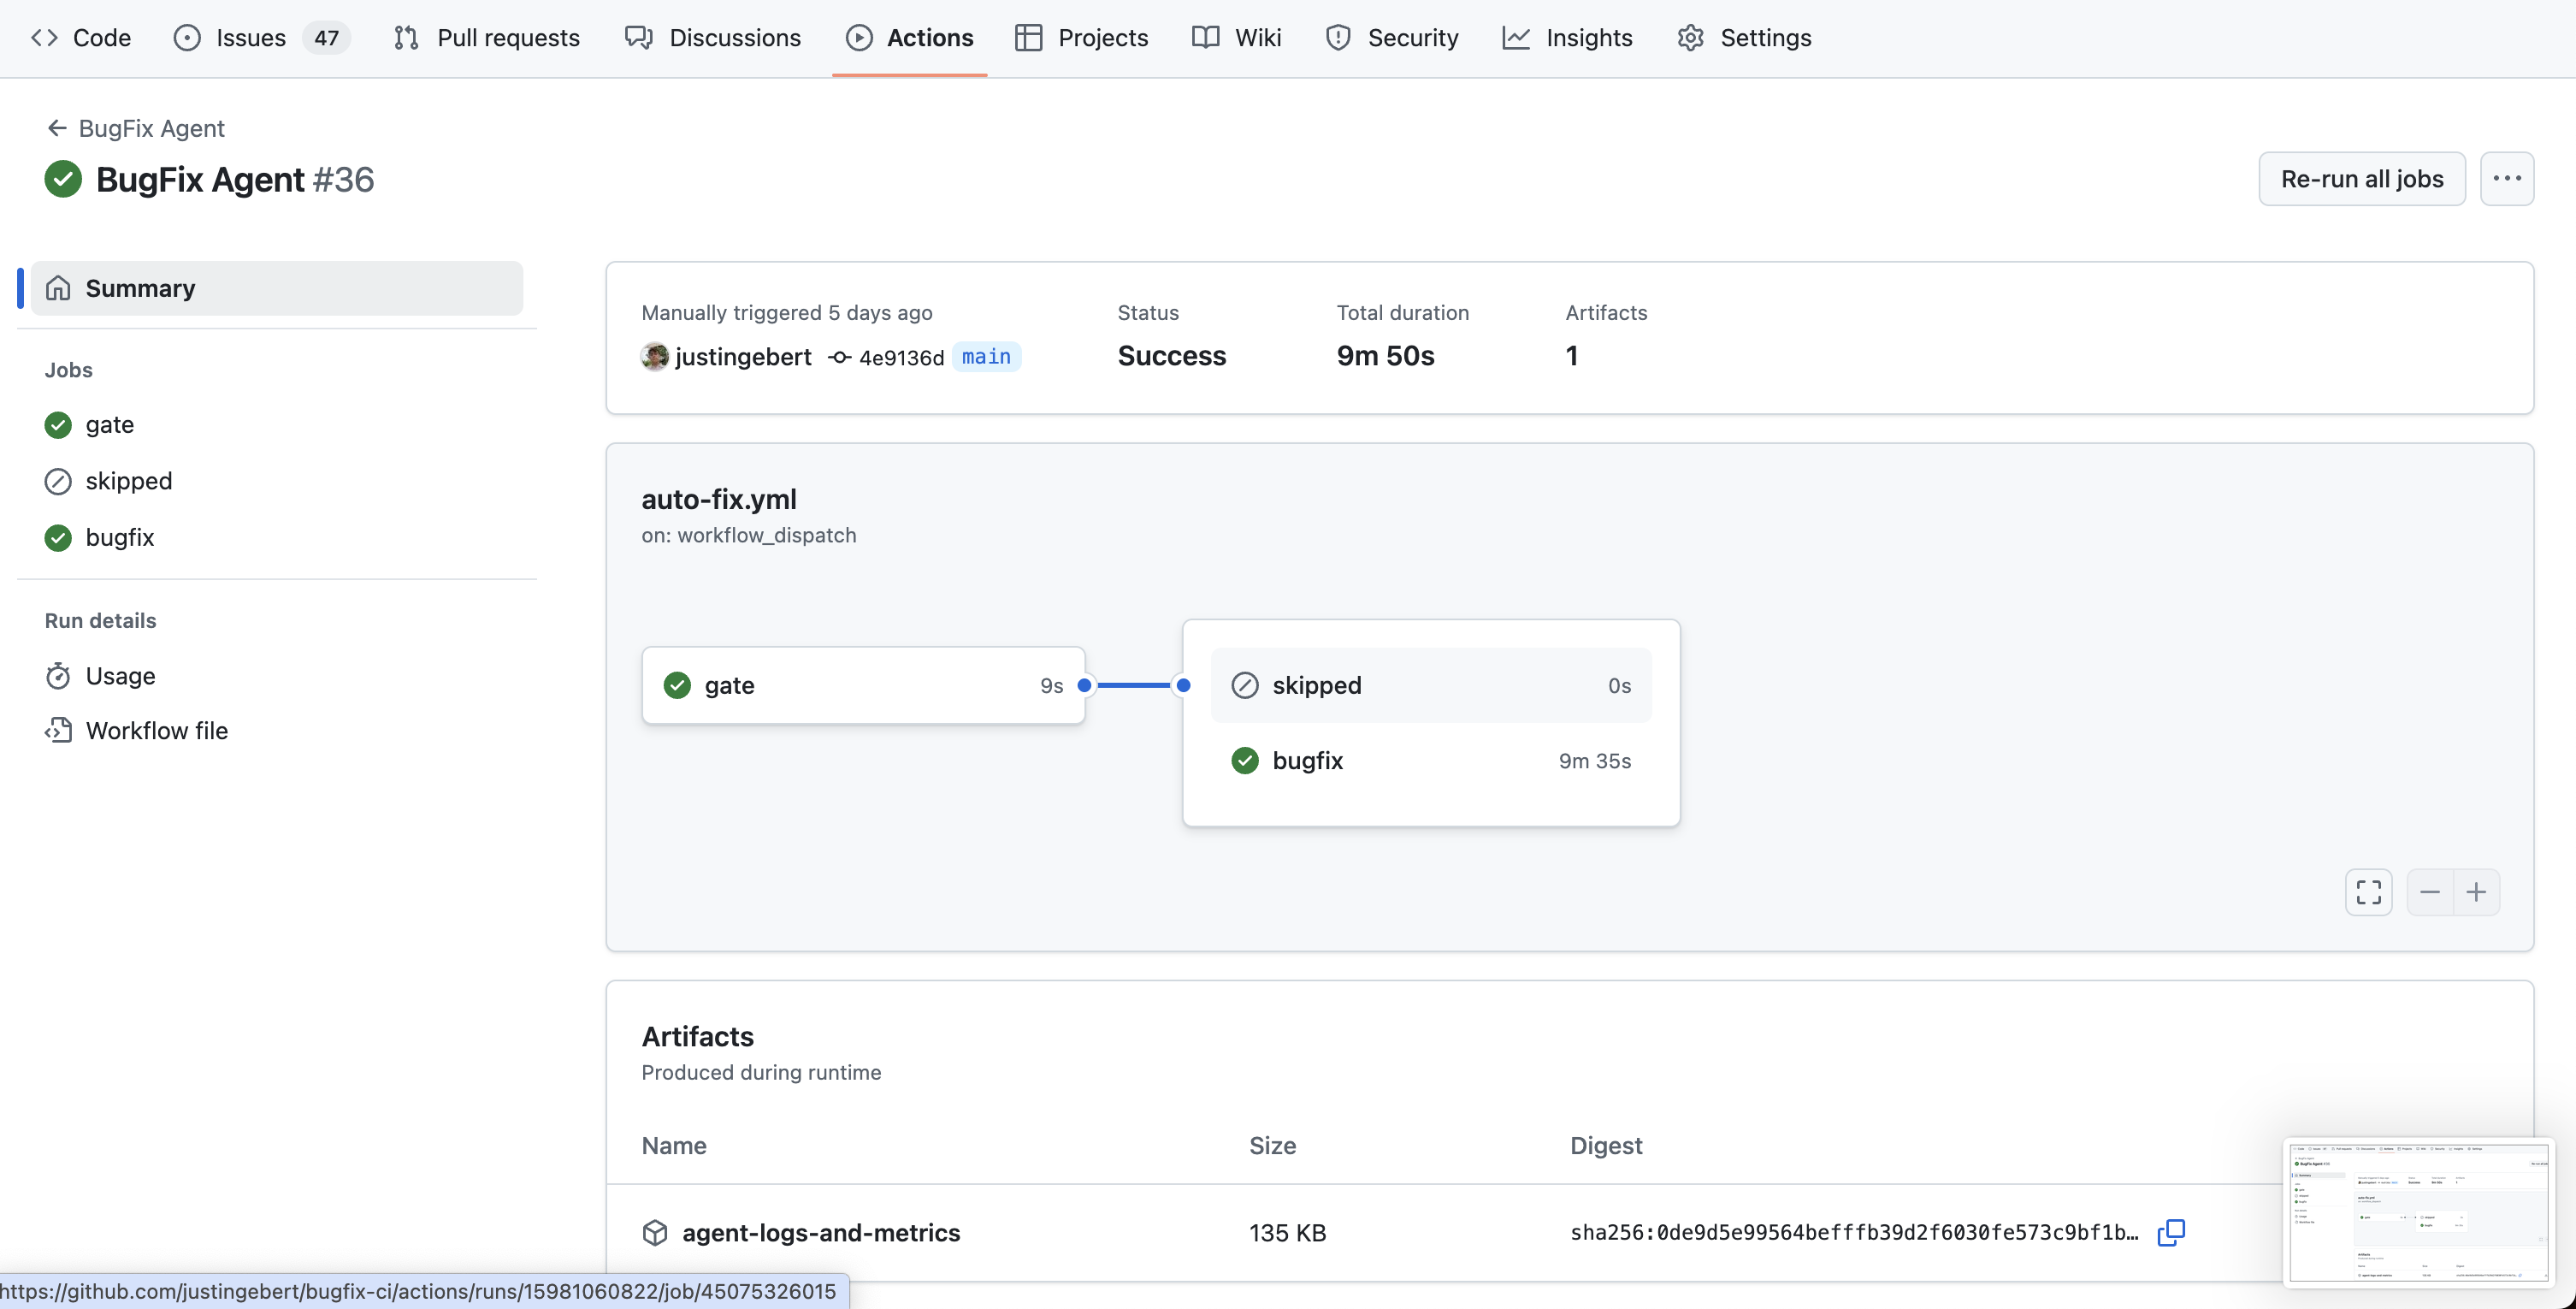
\includegraphics[width=1\textwidth]{images/workflow/Action.png}
    \caption{GitHub Action Run}
    \label{fig:apr-action}
\end{figure}

A run can produce two possible outcomes for each issue it processes. On a successful repair attempt it will create a pull request with the changes made to the codebase and the issue it is related to. This allows for easy review and merging of the changes into the main branch. The pull request will also contain information about the issue that was fixed, making it easy to track the changes made to the codebase.
\begin{figure}[H]
    \centering
    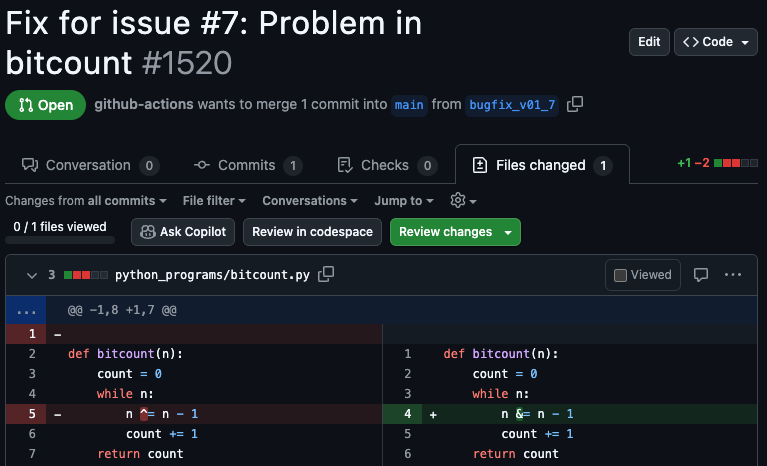
\includegraphics[width=1\textwidth]{images/workflow/PR.png}
    \caption{Resulting Pull Request}
    \label{fig:pr}
\end{figure}

When a repair attempt fails for an issue that is processed the failure is reported to the issue and the issues is labeled as failed so it wont be picked up again. This allows for easy tracking of issues that could not be fixed by the APR system.
\begin{figure}[H]
    \centering
    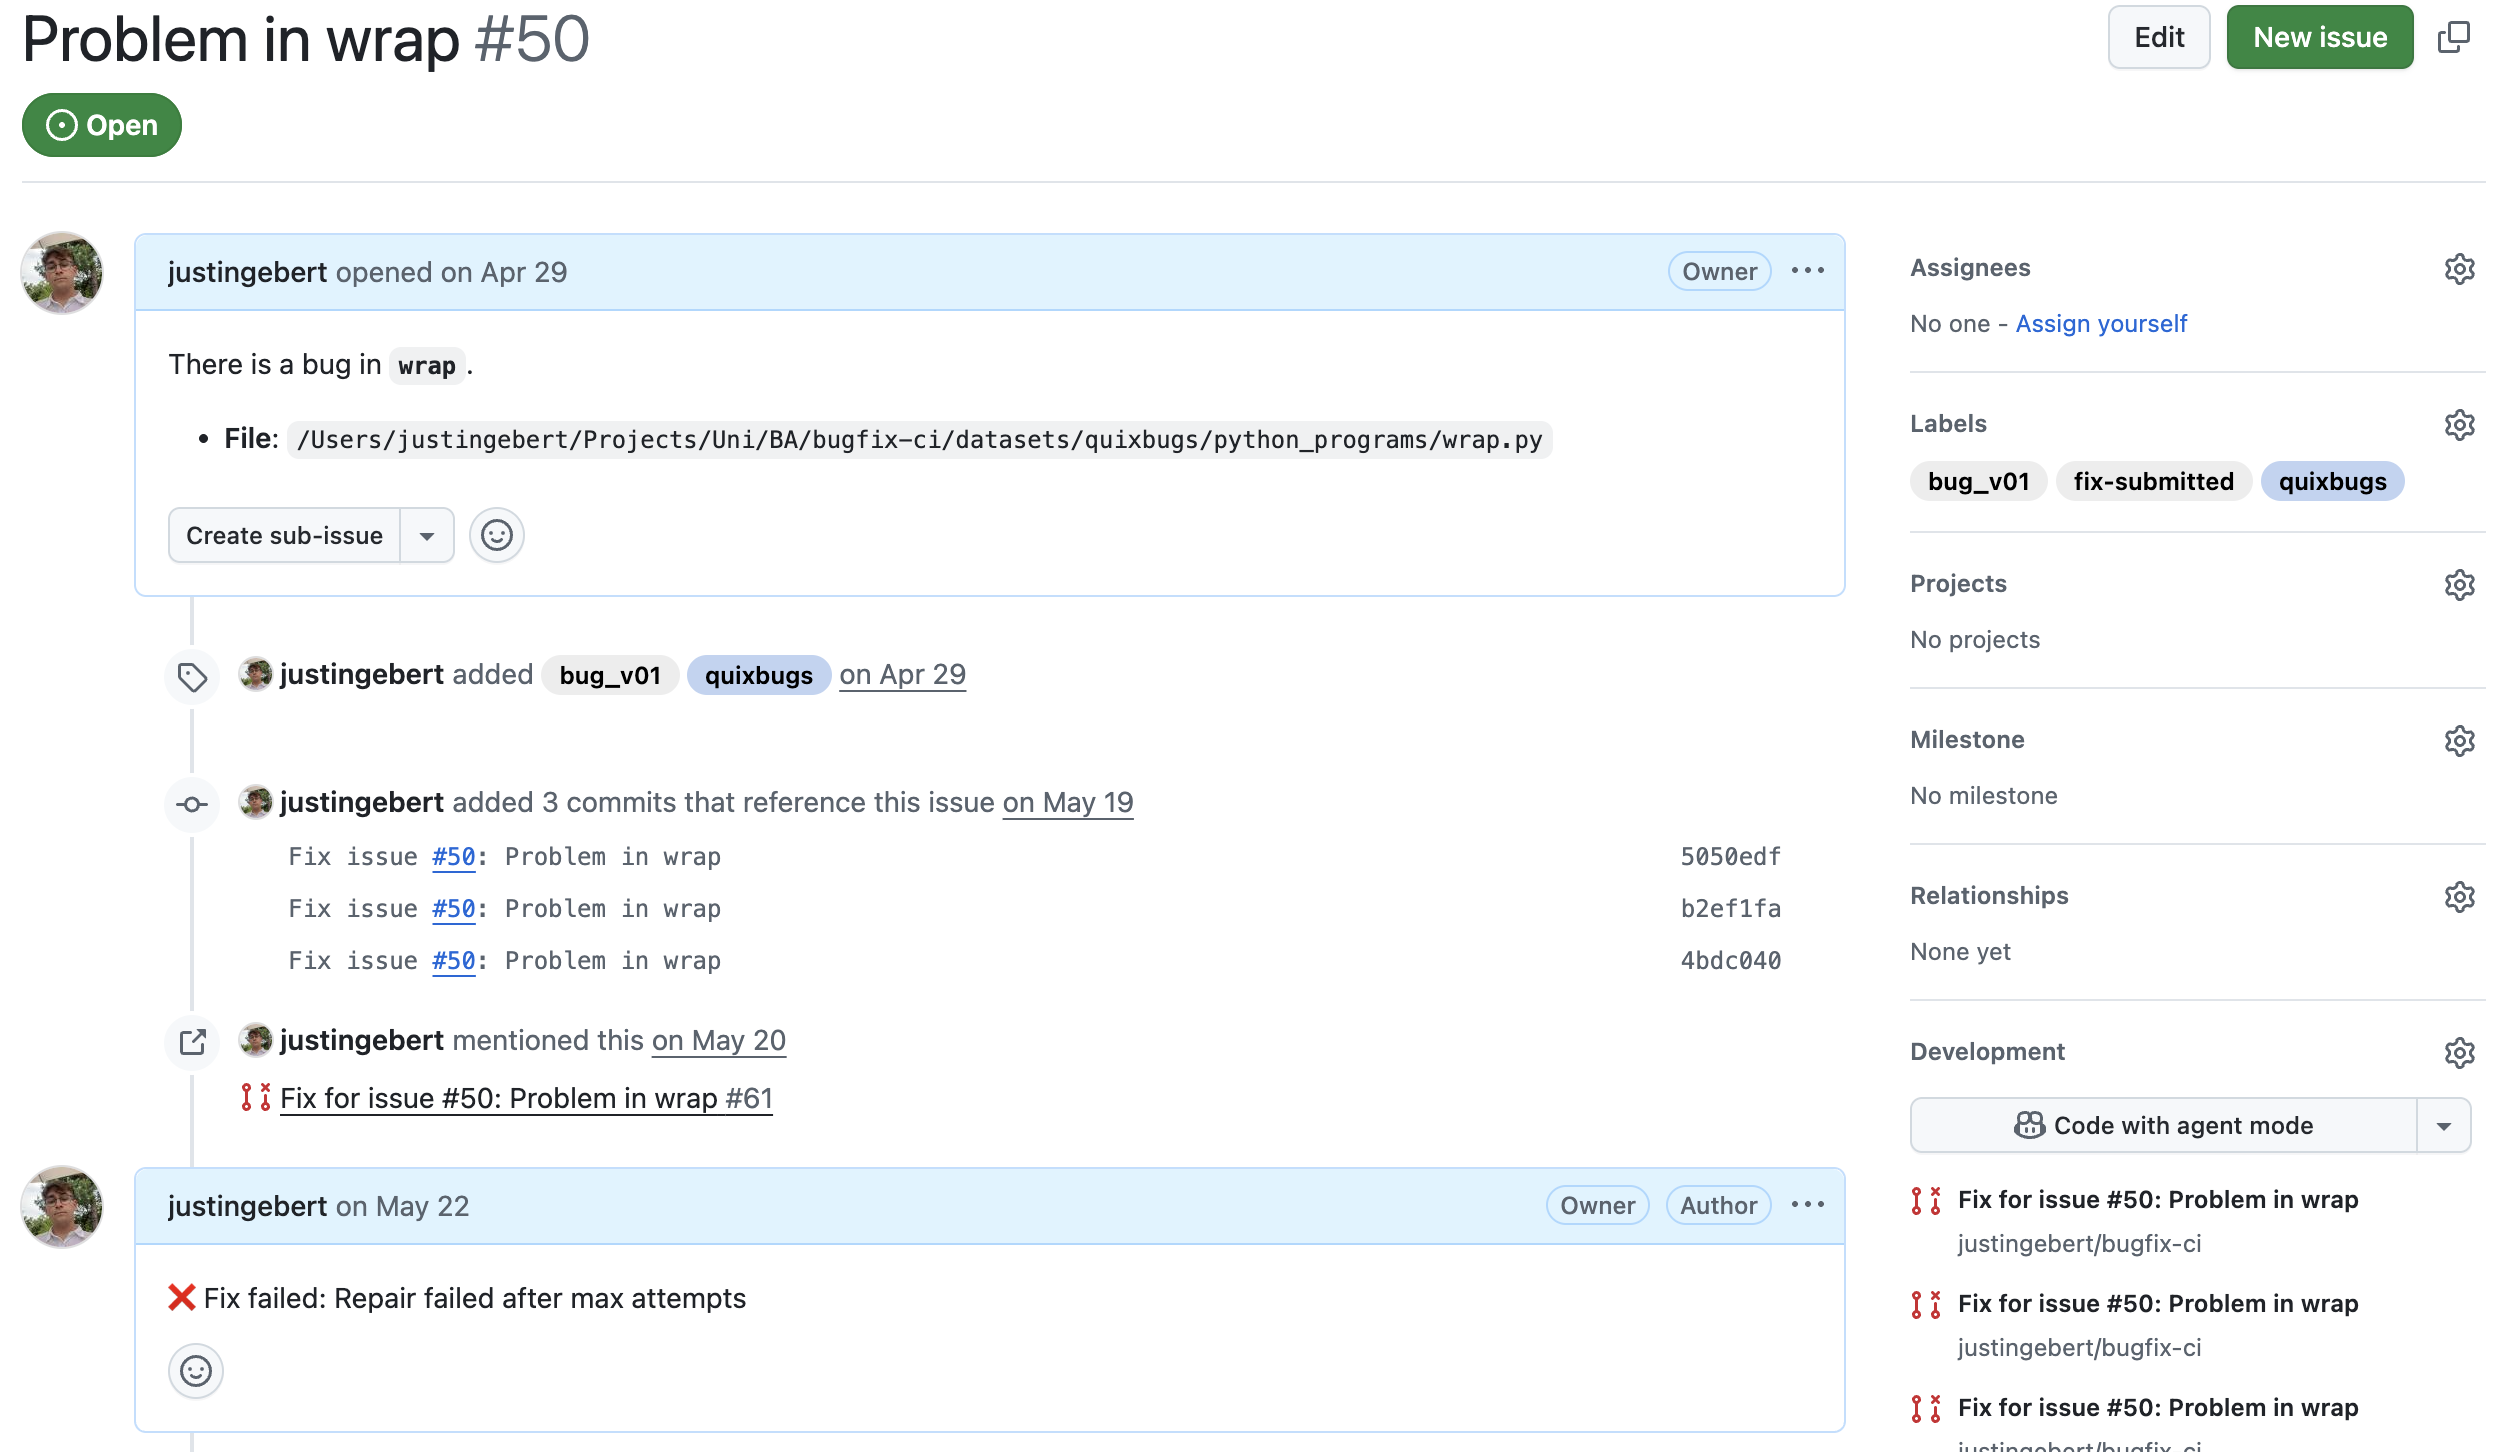
\includegraphics[width=1\textwidth]{images/workflow/issue comment.png}
    \caption{Failure Report}
    \label{fig:failure-report}
\end{figure}

When a new comment containing context gets added to the issue the APR system will automatically pick up the issue again. This allows for a more dynamic approach to bug fixing, where issues can be fixed as new information becomes available.

For transparency and debugging, each run provides a live log stream in the GitHub Actions tab. This allows users to see the progress of the run and any errors that occur during the execution. For further analysis logs, metrics and the context are also stored as artifacts to download.
\begin{figure}[H]
    \centering
    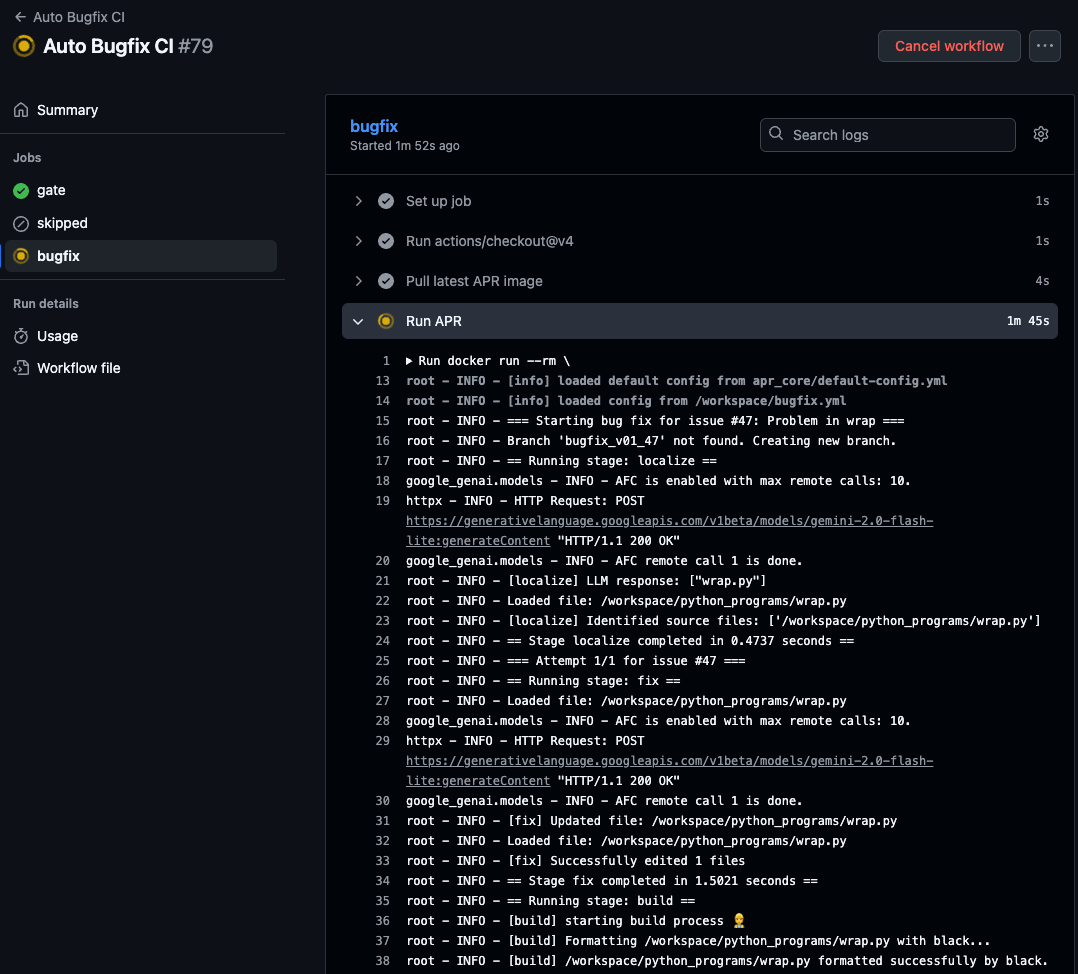
\includegraphics[width=1\textwidth]{images/workflow/logs.png}
    \caption{APR log stream}
    \label{fig:log-stream}
\end{figure}

In figure \ref{fig:flow} we can see the resulting flow diagram of the APR system. The diagram shows the steps taken by the user which have an effect on the state of the system and the steps taken by the system itself.
%TODO rework image
\begin{figure}[H]
    \centering
    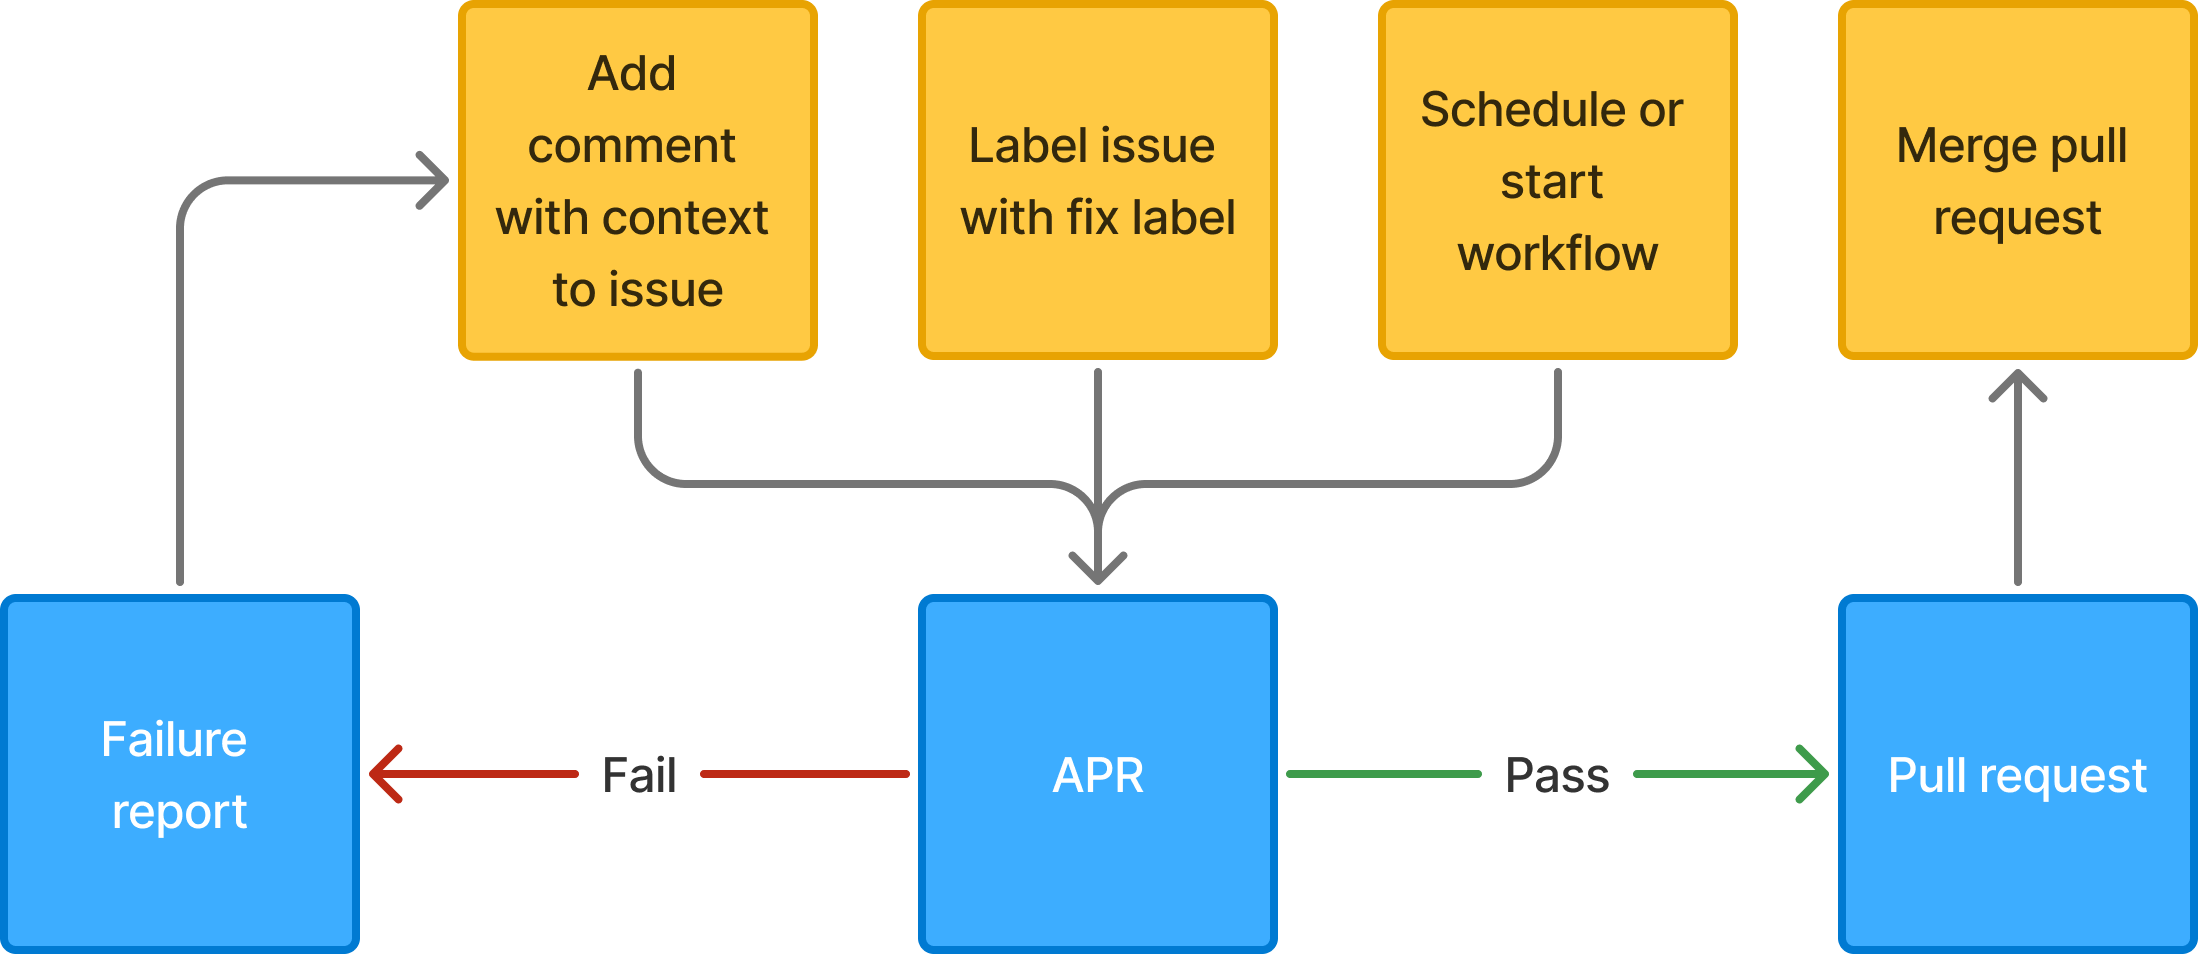
\includegraphics[width=0.9\textwidth]{images/flowcharts/flowresult.png}
    \caption{Resulting flow diagram}
    \label{fig:flow}
\end{figure}

\section{Evaluation Results}
In this section we will present the results of the quantitative evaluation of the APR prototype. This evaluation is based on the data collected and calculated for each run of the prototype \ref{table:run-metrics}.

\subsection{Validity}
- github runners have a lot of computational noise
- only small set of runs.

more regarding validity of results in section \ref{section:validity}.

\subsection{Baseline of Evaluation}
For the evaluation we executed the APR prototype on the repository containing 40 issues from the QuixBugs benchmark. \ref{subsection:environment-setup}. To evaluate effectiveness, performance and cost we evaluate the APR prototype using 12 different LLMs model defined in \ref{subsection:llm-selection}. This resulted in X pipelines runs each processing all 40 issues from the repository.
\subsection{Results}
The results of the evaluation are summarized in \ref{table:results}.

For testing the impact of the retry loop we collected the values with the retry loop enabled and disabled. The results are shown in \ref{table:retry-results}.

The table shows the repair success rate, average cost and average execution time for each model used in the evaluation.

\begin{table}[ht]
    \centering
    \small
    \begin{tabular*}{\textwidth}{@{\extracolsep{\fill}} p{3.5cm} | p{3cm} | p{3cm} | p{3cm} @{}}
        \hline
        \textbf{Model} & \textbf{Repair Success Rate} & \textbf{Average Cost Per Issue} & \textbf{Average Execution Time in seconds} \\
        \hline
        \textbf{gemini-2.0-flash-lite} & 85\% & \$0.0001 & 6.65s \\
        \textbf{gemini-2.0-flash} & 90\% & \$0.0002 & 7.63s \\
        \textbf{gemini-2.5-flash-lite-preview} & 67.5\% & \$0.0002 & 15.46s \\
        \textbf{gemini-2.5-flash} & 87.5\% & \$0.00096318 & 19.82s \\
        \textbf{gemini-2.5-pro} & 100\% & \$0.00 & 0.00s \\
        \textbf{gpt-4.1-nano} & 0.00\% & \$0.00  & 0.00s \\
        \textbf{gpt-4.1-mini} & 0.00\% & \$0.00 & 0.00s \\
        \textbf{gpt-4.1} & 0.00\% & 0.00 & \$0.00  \\
        \textbf{o4-mini} & 0.00\% & 0.00 & \$0.00  \\
        \textbf{claude-3-haiku} & 0.00\% & \$0.00  \\
        \textbf{claude-3-5-haiku} & 0.00\% & \$0.00 & 0.00 \\
        \textbf{claude-3-7-sonnet} & 0.00\% & \$0.00 & 0.00 \\
        \textbf{claude-sonnet-4-0} & 0.00\% & \$0.00 & 0.00 \\
        \hline
    \end{tabular*}
    \caption{Results of evaluation}
    \label{table:results}
\end{table}


The table shows the repair success rate, average cost, average number of attempts and average execution time for each model used in the evaluation.

\begin{table}[ht]
    \centering
    \small
    \begin{tabular*}{\textwidth}{@{\extracolsep{\fill}} p{3.5cm} | p{2cm} | p{2cm} | p{2cm} | p{2cm} @{}}
        \hline
        \textbf{Model} & \textbf{Repair Success Rate} & \textbf{Average Cost} & \textbf{Average Number of Attempts} & \textbf{Average Execution Time} \\
        \hline
        \textbf{gemini-2.0-flash} & 92.5\% & 0.00 & 0.00 & 0.00s \\
        \textbf{gemini-2.5-flash-lite} & 95\% & 0.00 & 0.00 & 0.00s \\
        \textbf{gemini-2.5-flash} & 0.00\% & 0.00 & 0.00 & 0.00s \\
        \textbf{gemini-2.5-pro} & 100\% & 0.00 & 0.00 & 0.00s \\
        \textbf{gpt-4.1-nano} & 0.00\% & 0.00 & 0.00 & 0.00s \\
        \textbf{gpt-4.1-mini} & 0.00\% & 0.00 & 0.00 & 0.00s \\
        \textbf{gpt-4.1} & 0.00\% & 0.00 & 0.00 & 0.00s \\
        \textbf{o4-mini} & 0.00\% & 0.00 & 0.00 & 0.00s \\
        \textbf{claude-3-haiku} & 0.00\% & 0.00 & 0.00 & 0.00s \\
        \textbf{claude-3-5-haiku} & 0.00\% & 0.00 & 0.00 & 0.00s \\
        \textbf{claude-3-7-sonnet} & 0.00\% & 0.00 & 0.00 & 0.00s \\
        \textbf{claude-sonnet-4-0} & 0.00\% & 0.00 & 0.00 & 0.00s \\
        \hline
    \end{tabular*}
    \caption{Results of evaluation with retry loop enabled}
    \label{table:retry-results}
\end{table}


Complete artifacts are available in the repository in the Appendix \ref{Appendix}.

